\documentclass[12pt, a4paper, oneside]{ctexart}
\usepackage{amsmath, amsthm, amssymb, bm, color, graphicx, geometry, mathrsfs,extarrows, braket, booktabs, array, xcolor, fontspec, appendix, float, subfigure, wrapfig, enumitem, titlesec, algorithm, mathtools}
\usepackage[colorlinks,linkcolor=red,anchorcolor=blue,citecolor=blue,urlcolor=blue,menucolor=black]{hyperref}

%%%% 设置中文字体 %%%%
% fc-list -f "%{family}\n" :lang=zh >d:zhfont.txt 命令查看已有字体
\setCJKmainfont[
    BoldFont=方正黑体_GBK,  % 黑体
    ItalicFont=方正楷体_GBK,  % 楷体
    BoldItalicFont=方正粗楷简体,  % 粗楷体
    Mapping = fullwidth-stop  % 将中文句号“.”全部转化为英文句号“.”,
]{方正书宋简体}  % !!! 注意在Windows中运行请改为“方正书宋简体.ttf” !!!
%%%% 设置英文字体 %%%%
\setmainfont{Minion Pro}
\setsansfont{Calibri}
\setmonofont{Consolas}

%%%% 设置代码块 %%%%
% 在vscode中使用minted需要先配置python解释器, Ctrl+Shift+P, 输入Python: Select Interpreter选择安装了Pygments的Python版本. 再在setting.json中xelatex和pdflatex的参数中加入 "--shell-escape", 即可
% TeXworks中配置方法参考: https://blog.csdn.net/RobertChenGuangzhi/article/details/108140093
\usepackage{minted}
\renewcommand{\theFancyVerbLine}{
    \sffamily\textcolor[rgb]{0.5,0.5,0.5}{\scriptsize\arabic{FancyVerbLine}}} % 修改代码前序号大小
% 加入不同语言的代码块
\newmintinline{cpp}{fontsize=\small, linenos, breaklines, frame=lines}
\newminted{cpp}{fontsize=\small, baselinestretch=1, linenos, breaklines, frame=lines}
\newmintedfile{cpp}{fontsize=\small, baselinestretch=1, linenos, breaklines, frame=lines}
\newmintinline{matlab}{fontsize=\small, linenos, breaklines, frame=lines}
\newminted{matlab}{fontsize=\small, baselinestretch=1, mathescape, linenos, breaklines, frame=lines}
\newmintedfile{matlab}{fontsize=\small, baselinestretch=1, linenos, breaklines, frame=lines}
\newmintinline{python}{fontsize=\small, linenos, breaklines, frame=lines, python3}  % 使用\pythoninline{代码}
\newminted{python}{fontsize=\small, baselinestretch=1, linenos, breaklines, frame=lines, python3}  % 使用\begin{pythoncode}代码\end{pythoncode}
\newmintedfile{python}{fontsize=\small, baselinestretch=1, linenos, breaklines, frame=lines, python3}  % 使用\pythonfile{代码地址}

%%%% 设置行间距与页边距 %%%%
\linespread{1.2}
\geometry{left=2.5cm, right=2.5cm, top=2.5cm, bottom=2.5cm}
% \geometry{left=1.84cm,right=1.84cm,top=2.18cm,bottom=2.18cm}  % 更小的页边距

%%%% 定理类环境的定义 %%%%
\newtheorem{example}{例}            % 整体编号
\newtheorem{theorem}{定理}[section] % 定理按section编号
\newtheorem{definition}{定义}
\newtheorem{axiom}{公理}
\newtheorem{property}{性质}
\newtheorem{proposition}{命题}
\newtheorem{lemma}{引理}
\newtheorem{corollary}{推论}
\newtheorem{condition}{条件}
\newtheorem{conclusion}{结论}
\newtheorem{assumption}{假设}
% \numberwithin{equation}{section}  % 公式按section编号 (公式右端的小括号)
% \newtheorem{algorithm}{算法}

%%%% 自定义环境 %%%%
\newsavebox{\nameinfo}
\newenvironment{myTitle}[1]{
    \begin{center}
    {\zihao{-2}\bf #1\\}
    \zihao{-4}\it
}{\end{center}}  % \begin{myTitle}{标题内容}作者信息\end{myTitle}
\newcounter{problem}  % 问题序号计数器
\newenvironment{problem}[1][]{\stepcounter{problem}\par\noindent\textbf{题目\arabic{problem}. #1}}{\smallskip\par}
\newenvironment{solution}[1][]{\par\noindent\textbf{#1解答. }}{\smallskip\par}  % 可带一个参数表示题号\begin{solution}{题号}
\newenvironment{note}{\par\noindent\textbf{注记. }}{\smallskip\par}
\newenvironment{remark}{\begin{enumerate}[label=\textbf{注\arabic*.}]}{\end{enumerate}}
%\BeforeBeginEnvironment{minted}{\vspace{-0.5cm}}  % 缩小minted环境距上文间距
%\AfterEndEnvironment{minted}{\vspace{-0.2cm}}  % 缩小minted环境距下文间距

%%%% 自定义段落开头序号,间距 (titlesec) %%%%
% 中文序号:\zhnum{section}, 阿拉伯序号:\arabic
\titleformat{\section}{\Large\bfseries}{\arabic{section}}{1em}{}[]
\titlespacing{\section}{0pt}{1.2ex plus .0ex minus .0ex}{.6ex plus .0ex}
\titlespacing{\subsection}{0pt}{1.2ex plus .0ex minus .0ex}{.6ex plus .0ex}
\titlespacing{\subsubsection}{0pt}{1.2ex plus .0ex minus .0ex}{.6ex plus .0ex}

%%%% 图片相对路径 %%%%
\graphicspath{{figures/}} % 当前目录下的figures文件夹, {../figures/}则是父目录的figures文件夹
\setlength{\abovecaptionskip}{-0.2cm}  % 缩紧图片标题与图片之间的距离
\setlength{\belowcaptionskip}{0pt} 

%%%% 缩小item,enumerate,description两行间间距 %%%%
\setenumerate[1]{itemsep=0pt,partopsep=0pt,parsep=\parskip,topsep=5pt}
\setitemize[1]{itemsep=0pt,partopsep=0pt,parsep=\parskip,topsep=5pt}
\setdescription{itemsep=0pt,partopsep=0pt,parsep=\parskip,topsep=5pt}

%%%% 自定义公式 %%%%
\everymath{\displaystyle} % 默认全部行间公式, 想要变回行内公式使用\textstyle
\DeclareMathOperator*\uplim{\overline{lim}}     % 定义上极限 \uplim_{}
\DeclareMathOperator*\lowlim{\underline{lim}}   % 定义下极限 \lowlim_{}
\DeclareMathOperator*{\argmax}{arg\,max}  % 定义取最大值的参数 \argmax_{}
\DeclareMathOperator*{\argmin}{arg\,min}  % 定义取最小值的参数 \argmin_{}
\let\leq=\leqslant % 简写小于等于\leq (将全部leq变为leqslant)
\let\geq=\geqslant % 简写大于等于\geq (将全部geq变为geqslant)
\DeclareRobustCommand{\rchi}{{\mathpalette\irchi\relax}}
\newcommand{\irchi}[2]{\raisebox{\depth}{$#1\chi$}} % 使用\rchi将\chi居中

%%%% 一些宏定义 %%%%
\def\bd{\boldsymbol}        % 加粗(向量) boldsymbol
\def\disp{\displaystyle}    % 使用行间公式 displaystyle(默认)
\def\tsty{\textstyle}       % 使用行内公式 textstyle
\def\sign{\text{sign}}      % sign function
\def\wtd{\widetilde}        % 宽波浪线 widetilde
\def\R{\mathbb{R}}          % Real number
\def\N{\mathbb{N}}          % Natural number
\def\Z{\mathbb{Z}}          % Integer number
\def\Q{\mathbb{Q}}          % Rational number
\def\C{\mathbb{C}}          % Complex number
\def\K{\mathbb{K}}          % Number Field
\def\P{\mathbb{P}}          % Polynomial
\def\E{\mathbb{E}}          % Exception
\def\d{\mathrm{d}}          % differential operator
\def\e{\mathrm{e}}          % Euler's number
\def\i{\mathrm{i}}          % imaginary number
\def\re{\mathrm{Re}}        % Real part
\def\im{\mathrm{Im}}        % Imaginary part
\def\res{\mathrm{Res}}      % Residue
\def\ker{\mathrm{Ker}}      % Kernel
\def\vspan{\mathrm{vspan}}  % Span  \span与latex内核代码冲突改为\vspan
\def\L{\mathcal{L}}         % Loss function
\def\O{\mathcal{O}}         % big O notation
\def\wdh{\widehat}          % 宽帽子 widehat
\def\ol{\overline}          % 上横线 overline
\def\ul{\underline}         % 下横线 underline
\def\add{\vspace{1ex}}      % 增加行间距
\def\del{\vspace{-1.5ex}}   % 减少行间距

\makeatletter
\newenvironment{breakablealgorithm}
  {% \begin{breakablealgorithm}
   \begin{center}
     \refstepcounter{algorithm}% New algorithm
     \hrule height.8pt depth0pt \kern2pt% \@fs@pre for \@fs@ruled
     \renewcommand{\caption}[2][\relax]{% Make a new \caption
       {\raggedright\textbf{\fname@algorithm~\thealgorithm} ##2\par}%
       \ifx\relax##1\relax % #1 is \relax
         \addcontentsline{loa}{algorithm}{\protect\numberline{\thealgorithm}##2}%
       \else % #1 is not \relax
         \addcontentsline{loa}{algorithm}{\protect\numberline{\thealgorithm}##1}%
       \fi
       \kern2pt\hrule\kern2pt
     }
  }{% \end{breakablealgorithm}
   \end{center}
  }
\makeatother

%%%% 正文开始 %%%%
\begin{document}

%%%% 以下部分是正文 %%%%  
\clearpage
\begin{myTitle}{机器学习实验报告}
    强基数学002\ 吴天阳\ 2204210460
\end{myTitle}
本报告包含K-均值聚类、混合高斯(GMM)、去偏变分自动编码机(DB-VAE)三个实验部分,
每个部分的完整算法代码均在代码文件夹\texttt{./code}下给出。
\section{K-均值聚类}
设数据集为$\{\bd{x}_1,\cdots,\bd{x}_N\},\ \bd{x}_i\in\R^D$,由$N$个在$\R^D$中的观测值构成。K-均值聚类(K-means Clustering)的目标是将数据集划分为$K$簇(Cluster),
假设$\bd{\mu}_k\in\R^D,\ (k=1,\cdots,K)$代表簇的中心,我们的目标是最小化每个数据点到最近$\bd{\mu}_k$的距离平方和。

为方便描述每个数据点的分类,引入二进制指标集$r_{nk}\in\{0,1\}$,如果数据点$\bd{x}_n$分配到簇$k$,那么$r_{nk} = 1$且$r_{nj}=0,\ (j\neq k)$。
根据该编码方法,可以定义以下最小化目标\textbf{失真度量(distortion measure)}:
\begin{equation}\label{eq-kmeansJ}
    J = \sum_{n=1}^N\sum_{k=1}^Kr_{nk}||\bd{x}_n-\bd{\mu}_k||^2
\end{equation}
K-均值聚类也是用了EM算法,首先给出如何划分为EM算法:
\begin{itemize}
    \item E步:固定$\mu_k$,求使得$J$最小化的$r_{nk}$(求出期望)。
    \item M步:固定$r_{nk}$,求使得$J$最小化的$\mu_k$(最大化)。
\end{itemize}
\paragraph{E步}当固定$\mu_k$时,由于$J$关于$r_{nk}$是线性的,即不同的数据$\bd{x}_n$之间相互独立,所以可以对于每个样本单独进行优化,对于样本$\bd{x}_n$的$r_{nk}$满足求解以下最优化问题:
\begin{equation*}
    \begin{aligned}
        \min_{r_{nk}\in\{0,1\}}&\ \sum_{k=1}^Kr_{nk}||\bd{x}_n-\bd{\mu}_k||^2\\
        s.t.&\ \sum_{k=1}^Kr_{nk} = 1
    \end{aligned}\Rightarrow r_{nk} = \begin{cases}
        1, &\text{当}\ k=\argmin_{1\leq j\leq K}||\bd{x}_n-\bd{\mu}_j||^2,\\
        0, &\text{否则}.
    \end{cases}
\end{equation*}
不难发现,最优化结果正好就表明只需将每个$\bd{x}_n$分配到最近的簇中心$\bd{\mu}_k$上。
\paragraph*{M步}当固定$r_{nk}$时,由于$J$是关于$\mu_k$的二次函数,所以可以通过导数为零确定最小化点:
\begin{equation*}
    2\sum_{n=1}^Nr_{nk}(\bd{x}_n-\bd{\mu}_k) = 0\Rightarrow \bd{\mu}_k=\frac{\disp\sum_{1\leq n\leq N}r_{nk}\bd{x}_n}{\disp\sum_{1\leq n\leq N}r_{nk}}
\end{equation*}
表达式中分母是簇$k$分配到的数据的个数,所以$\mu_k$的更新就是所有簇$k$分配到的数据点的平均值,因此被称为K-均值,算法总共两步:将每个数据点分配到最近的簇,
重新计算簇均值以替代新的簇。由于该方法每一步都会使得$J$单调递减,所以算法收敛性显然,但是它只能收敛到$J$的局部最小值。
\section{混合高斯模型}
混合高斯模型(Gaussian Mixture Model, GMM)是一种基于概率的聚类模型,首先我们可以将所有的变量均视为随机变量,包括观测变量$x$和隐变量$\theta,\omega$,
它们都服从某个概率分布,于是可以将模型参数求解转化为求解$p(\theta|D)$,即根据数据集$D$求出模型参数$\theta$的后验分布,所以可以用最大似然(MLE)方法求解。

用上述方法理解重新聚类问题:混合概率模型的隐变量就是$y$表示数据的类别种类,服从分布$p(y=k) = \pi_k$(表示全部的$\bd{x}$来自类别$k$的概率大小),
从\textbf{数据生成}的角度理解,第$k$个类别的数据$\bd{x}$应来自与$y$相关的某个分布$p(\bd{x}|y=k)$中(不妨令该分布为多维正态分布),
于是二者的联合分布为
\begin{equation*}
p(\bd{x},y) = p(y)p(\bd{x}|y) \xlongequal{y=k} \pi_k\mathcal{N}(\bd{x}|\bd{\mu}_k,\Sigma_k)   
\end{equation*}
通过联合分布我们又可以求出\textbf{数据预测}的结果:
\begin{equation*}
p(y|\bd{x}) = \frac{p(\bd{x},y)}{p(\bd{x})} \xlongequal{y=k} \frac{\pi_k\mathcal{N}(\bd{x}|\bd{\mu}_k,\Sigma_k)}{\sum_{k=1}^K\pi_k\mathcal{N}(\bd{x}|\bd{\mu}_k,\Sigma_k)}
\end{equation*}

将全部的参数简记为$\theta = (\mu_1,\cdots,\mu_K,\sigma^2,\pi_1,\cdots,\pi_K)$,于是关于$\theta$的MLE为
\begin{equation}\label{eq-MLE}
    \max_{\theta}\prod_{i=1}^Np(x_i|\theta) = \prod_{i=1}^N\sum_{k=1}^Kp(x_i,y_i=k|\theta) = \prod_{i=1}^N\sum_{k=1}^Kp(y_i=k|\theta)p(x_i|y_i=k,\theta)
\end{equation}
\subsection{由GMM导出K-均值}
我们考虑一个GMM的特殊情况,假设所有的方差均相同,即$\Sigma = \Sigma_k,\ (k=1,\cdots,K)$,并令$\pi_k = \frac{1}{n}\sum_{i=1}^nr_{nk}$,则$\bd{\mu}_k$似然函数为
\begin{align*}
    L =&\ \prod_{i=1}^{N}\sum_{k=1}^K\pi_kp(x_i) = \prod_{i=1}^{N}\sum_{k=1}^K\pi_k\mathcal{N}(x_i|\bd{\mu}_k,\Sigma)\\
    =&\ \prod_{i=1}^{N}\sum_{k=1}^K\pi_k(2\pi)^{-\frac{k}{2}}|\Sigma|^{-\frac{1}{2}}\exp\left\{-\frac{1}{2}(\bd{x}-\bd{\mu}_k)^T\Sigma^{-1}(\bd{x}-\bd{\mu}_k)\right\}
\end{align*}
取对数后得到MLE为
\begin{equation*}
    \max_{\bd{\mu}_k}-\sum_{i=1}^{N}\sum_{k=1}^K\pi_{k}||x_i-\bd{\mu}_k||^2 = \min_{\bd{\mu}_k}\sum_{i=1}^{N}\sum_{k=1}^K\pi_{k}||x_i-\bd{\mu}_k||^2
\end{equation*}
结果与K-均值(\ref{eq-kmeansJ})式中的失真度量$J$的区别仅需将$\pi_k$换为$r_{nk}$,而这个转换就会将聚类方法从GMM的\textbf{软分类}变为K-均值的\textbf{硬分类}。

其次我们可以利用GMM的预测方法证明:当方差相同时(K-均值的分类边界),分类边界是线性的。假设数据$\bd{x}$分到$i,j$类别具有相同的可能性时,也就是$p(y=i|\bd{x})=p(y=j|\bd{x})$,于是:
\begin{align*}
    0=&\ \log\frac{p(y=i|\bd{x})}{p(y=j|\bd{x})} = \log\frac{p(\bd{x}|y=i)\frac{p(y=i)}{p(\bd{x})}}{p(\bd{x}|y=j)\frac{p(y=j)}{p(\bd{x})}} = \log\frac{p(\bd{x}|y=i)\pi_i}{p(\bd{x}|y=j)\pi_j}\\
    =&\ \log\frac{\pi_i}{\pi_j} + ||\bd{x}-\bd{\mu}_i||^2 - ||\bd{x}-\bd{\mu}_j||^2 = \log\frac{\pi_i}{\pi_j} + 2(\bd{\mu}_j^T-\bd{\mu}_i^T)\bd{x}+\bd{\mu}_i^T\bd{\mu}_i - \bd{\mu}_i^T\bd{\mu}_j\\
    \Rightarrow&\  \bd{w}^T\bd{x} = \bd{b}
\end{align*}
说明如果$\bd{x}$分为类别$i,j$的可能性相同时,则$\bd{x}$一定处于直线$\bd{w}^T\bd{x}=\bd{b}$上。同理,对于一般情况$\Sigma_k$,计算得到的分类边界为$\bd{x}^TW\bd{x}+\bd{w}^T\bd{x}+\bd{c}$,
说明GMM的分类边界就是二次函数。
\subsection{使用EM算法进行参数求解}
观察(\ref{eq-MLE})式,对其取对数仍然无法将内部的求和符号展开成线性表示,所以难以求出极值,考虑基于$p(x,y)$求$\theta$的MLE:
\begin{align*}
    \max_{\theta}\prod_{i=1}^Np(\bd{x}_i,y_i|\theta)\propto\sum_{i=1}^N\log p(\bd{x}_i,y_i|\theta) = \sum_{i=1}^N\sum_{k=1}^Kp(y_i=k|\bd{x}_i,\theta)\log p(\bd{x}_i,y_i|\theta)
\end{align*}
\textbf{M步}:假设我们在$t-1$步已经得到了参数估计值$\theta^{t-1}$,于是可以在第$t$步建立$Q$函数,然后最大化该函数得到$\theta^t$
\begin{equation}\label{GMM-M}
    \max_{\theta^t}Q(\theta^t|\theta^{t-1}) = \sum_{i=1}^n\sum_{k=1}^Kp(y_i=k|\bd{x}_i,\theta^{t-1})\log p(\bd{x}_i,y_i=k|\theta^t)
\end{equation}
\textbf{E步}:就是在$t-1$步时,基于$\theta^{t-1}$计算数据$\bd{x}_i$从属于每个类别的概率:
\begin{equation*}
    R_{i,k}^{t-1} = p(y_i=k|\bd{x}_i,\theta^{t-1}) = \frac{\pi_k^{t-1}\mathcal{N}(\bd{x}_i|\bd{\mu}_k^{t-1},\Sigma_k^{t-1})}{\sum_{k=1}^K\pi_k^{t-1}\mathcal{N}(\bd{x}_i|\bd{\mu}_k^{t-1},\Sigma_k^{t-1})}
\end{equation*}
而E步的计算结果,就是M步中$Q$函数中$\log p(\bd{x}_i,y_i=k|\theta^t)$前的加权系数。

我们先不探讨上述方法的收敛性,通过Lagrange乘子法和令导数为零可以求解求解(\ref{GMM-M})式:
\begin{align}
    \text{由Lagrange乘子法:}
    \nonumber\nabla_{\pi_k^t}Q+\lambda\nabla_{\pi_k^t}\left(\sum_{k=1}^K\pi_k-1\right) = 0\Rightarrow&\ \frac{\sum_{i=1}^NR_{i,1}^{t-1}}{\pi_1^t} = \cdots=\frac{\sum_{i=1}^NR_{i,k}^{t-1}}{\pi_k^t}\\
    \nonumber\xRightarrow{\sum_{k=1}^KR_{i,k}^{t-1} = 1}&\ {\color{red}\pi_k^t = \frac{\sum_{i=1}^NR_{i,k}^{t-1}}{N}}\\
    \label{GMM-update}\nabla_{\bd{\mu}_k^t}Q = 0\Rightarrow \sum_{i=1}^NR_{i,k}^{t-1}(\bd{x}_i-\bd{\mu}_k^t) = 0\Rightarrow&\ {\color{red}\bd{\mu}_k^t = \sum_{i=1}^Nw_{ik}\bd{x}_i}\\
    \nonumber\nabla_{\Sigma_k^t}Q = 0\Rightarrow \sum_{i=1}^NR_{i,k}^{t-1}(-\Sigma_k^t + (\bd{x}_i-\bd{\mu}_k^t)^T(\bd{x}_i-\bd{\mu}_k^t)) = 0\Rightarrow&\ {\color{red}\Sigma_k^t = \sum_{i=1}^Nw_{ik}(\bd{x}_i-\bd{\mu}_k^t)^T(\bd{x}_i-\bd{\mu}_k^t)}
\end{align}
其中$w_{ik} = \frac{R_{i,k}^{t-1}}{\sum_{i=1}^NR_{i,k}^{t-1}}$。通过上式中的标红的部分,就可以得到第$t$步下的新参数值。
\subsection{EM算法收敛性证明}
首先引入一个求解函数极值的技术:若要求解$f(x)$的极小值,可以先取其定义域上任意一点$x_0$,再找到一个在$(x_0,f(x_0))$处与$f$相切的函数$g(x)$,并且要求$g(x)$是$f(x)$的上界,
令$x_1\gets \argmin_{x}g(x)$(求极大值反之亦然),根据该方法进行迭代即可得到$f(x)$的极小值点。

下面推到一个关于$\theta$的MLE重要结论,该方程成为\textbf{变分方程}:
\begin{align}
\label{eq-var}\log p(x|\theta) =&\ \int_Yq(y)\log p(x|\theta)\,\mathrm{d}y = \int_Yq(y)\log\frac{p(x,y|\theta)}{p(y|x,\theta)}\frac{q(y)}{q(y)}\,\mathrm{d}y\\
\nonumber =&\ \underbrace{\int_Yq(y)\log p(x,y|\theta)\,\mathrm{d}y}_{\text{核函数}} - \underbrace{\int_Yq(y)\log q(y)\,\mathrm{d}y}_{\text{与}\theta\text{无关}} + \underbrace{\int_Y q(y)\log\frac{q(y)}{p(y|x,\theta)}\,\mathrm{d}y}_{\text{KL}(q||p)}
\end{align}
注意到右边第三项正好是$p,q$的KL散度,于是有$\text{KL}(q||p) \geq 0$,于是前两项构成$\log p(x|\theta)$的下界,要求极大似然的极大值,第二项与$\theta$无关,所以只需对第一项求即可。
注意上式只讨论了一个数据,极大似然是对所有数据的对数似然求和得到:
\begin{equation*}
    \max_{\theta}\sum_{i=1}^N\int_Yq(y)\log p(\bd{x}_i,y|\theta)\,\d y
\end{equation*}
于是当我们取$q(y) = p(y|\bd{x},\theta)$时,KL散度正好为$0$,极大似然对应的$\theta^*$可以通过以下迭代式求解:
\begin{equation*}
    \theta^*\gets\argmax_{\theta^*}\sum_{i=1}^N\int_Yp(y|\bd{x}_i,\theta)\log p(\bd{x}_i,y|\theta^*)\,\d y
\end{equation*}
将积分号换为求和符号就可以得到EM算法中M步的(\ref{GMM-M})式。由上面引入的函数极值求解技术,可以证明每次EM都可以使得MLE下降,从而达到极小值点,说明EM算法具有收敛性。
\section{变分自动编码机}
\subsection{基本思想}
变分自动编码机(Variational AutoEncoder, VAE),是一种通过完全无监督的方式学习数据中的潜在特征编码。参考论文\href{https://arxiv.org/pdf/1312.6114.pdf}{Auto-Encoding Variational Bayes}。

设隐参数维数为$K$,记数据$\bd{x}$对应的真实隐参数为$\bd{z}\in\R^K$。基于所有变量都服从某个参数分布的思路,我们可以定义以下两个分布函数:
\begin{itemize}
    \item $q_\phi(\bd{z}) = q(\bd{z}|\bd{x},\phi)$称为\textbf{编码分布},该网络的输入为数据$\bd{x}$,通过网络参数$\phi$,估计出隐参数$\bd{z}$的分布。
    \item $p_\theta(\bd{x}) = p(\bd{x}|\bd{z},\theta)$称为\textbf{解码分布},该网络的输入为隐参数$\bd{z}$,通过网络参数$\theta$,得到重建数据$\hat{\bd{x}}$的分布。
\end{itemize}
\textbf{注}:上面两个函数均为概率密度函数,输入为随机变量,输出为对应的概率值;而非神经网络函数,如果要表示编码神经网络,记法不变,则\textbf{编码网络}为$q_{\phi}(\bd{x})$,\textbf{解码网络}为$p_{\theta}(\bd{z})$。
还需注意,由于我们无法通过神经网络得到随机变量$\bd{z}$的分布,所以我们只能假设其服从正态分布$\mathcal{N}(\bd{\mu},\sigma^2I)$,并将编码网络的输出设置为$K+1$维,其中前$K$维表示$\bd{z}$的均值$\bd{\mu}$,最后一维表示方差$\sigma$(或者$\log \sigma$).

为了能够优化上述参数$\phi,\theta$,我们需要找到与之相关的损失函数,由于是概率参数优化,不难想到使用MLE,于是仍然可以从变分方程(\ref{eq-var})式出发,可以得到:
\begin{equation*}
    \log p(\bd{x}|\theta) = \underbrace{\text{KL}(q_{\phi}(z)||p_\theta(z))}_{\text{KL散度}} + \underbrace{\int q_\phi(z)\log\frac{p_\theta(x,z)}{q_\phi(z)}\,\d z}_{\text{变分下界}L}
\end{equation*}
由于KL散度恒大于零,所以第二项$L$就是$\log p(\bd{x}|\theta)$的下界,如果要最大化似然$\log p(\bd{x}|\theta)$,也就是最大化$L$,于是
\begin{align*}
    \max_{\phi,\theta}L =&\ \int q_\phi(z)\log\frac{p(z)p_\theta(x)}{q_\phi(z)}\,\d z = -\int q_\phi(z)\log\frac{q_\phi(z)}{p(z)}+\int q_\phi(z)\log p_\theta(x)\,\d z\\
    =&\ -\text{KL}(q_{\phi}(z)||p(z)) + \E_{q_{\phi}(z)}\left[\log p_{\theta}(x|z)\right]
\end{align*}
于是MLE等价于:最小化$q_\phi(z)$与$\mathcal{N}(0,I)$的KL散度,我们可以直接计算出两个正态分布的KL散度,
将这部分称为\textbf{隐变量损失}:
\begin{equation*}
    L_{KL}:= \text{KL}(q_{\phi}(z)||p(z)) = \frac{1}{2}\sum_{i=1}^B(\sigma_i + \mu_i^2-1-\log\sigma_i)
\end{equation*}

最大化第二项$\E_{q_{\phi}(z)}\left[\log p_{\theta}(x|z)\right]$等价于最小化输入的数据与重建结果的误差,
可以使用最小化$\ell^1$或$\ell^2$范数代替,这部分称为\textbf{重建损失}$L_{\bd{x}}(\bd{x},\hat{\bd{x}})$,
下面我们用$\ell^1$范数表示输入与输出的误差,则
\begin{equation*}
    L_{\bd{x}}(\bd{x},\hat{\bd{x}}) := ||\bd{x}-\hat{\bd{x}}||_1
\end{equation*}

综上,VAE的损失函数为
\begin{equation}\label{eq-vae-loss}
    L_{\text{VAE}} = c\cdot L_{KL} + L_{\bd{x}}(\bd{x},\hat{\bd{x}})
\end{equation}
如果将KL散度理解为正则化项,则其中的$c$为KL正则化系数。
\subsubsection{参数重采样技巧}
VAE需要使用“参数重采样技巧”(Reparameterization Trick)对隐变量进行采样,这是因为我们在使用梯度下降对参数进行优化时,
在解码部分出现了随机变量$\bd{z}$,即$p_{\theta}(\bd{x}|\bd{z})$,这样会导致梯度下降无法进行,考虑用观测值对其进行估计;
由于$\bd{z}\sim q_{\phi}(\bd{z}|\bd{x})$,于是我们可以通过对$\bd{z}$的采样结果进行梯度计算。

在\textbf{VAE基本思想}中注释部分说明了编码网络可以得到$\bd{z}$的分布参数$\bd{\mu},\sigma$,所以可以通过标准正态分布的采样$\sigma\sim\mathcal{N}(0,I)$进行缩放平移得到$\bd{z}$的采样:
\begin{equation*}
    \bd{z} = \bd{\mu} + \sigma\varepsilon = \bd{\mu}+\exp\left\{\frac{1}{2}\log(\sigma^2I)\right\}\varepsilon
\end{equation*}
写成$\log\sigma$的形式只是因为在实际预测网络中,直接预测标准差可能误差较大,所以对标准差做对数变换。

\subsection{去偏自动编码机}
去偏变分自动编码机(Debiasing Variational AutoEncoder, DB-VAE)在VAE基础上对训练数据的选取上做了一点改进,
从而可以一定程度上避免数据集的偏差导致模型的偏差。

具体来讲:它通过自适应重采样(自动选择数据,
进行重复性训练)减轻训练集中的潜在偏差. 例如:面部识别训练集中,大多数图片的
人脸都是正面图像,而侧脸的图像偏少,如果将它们均等地训练,训练出的模型可能对
正脸识别效果优于侧脸的效果,这就是数据偏差(Debiasing). 为了平衡这种偏差有两
种方法,一是使用人工处理,提高数据集中偏差数据的训练数量,但操作十分复杂,而
且人无法判断哪些数据是偏差数据;二是通过机器自动识别偏差数据,然后自我调整数
据的训练数量,这就是 DB-VAE 的提升之处.

DB-VAE 的示意图如图所示,图片来源
论文\href{http://introtodeeplearning.com/AAAI_MitigatingAlgorithmicBias.pdf}{Uncovering and Mitigating Algorithmic Bias through Learned Latent Structure}.
\begin{figure}[htbp]
    \centering
    \includegraphics[scale=0.4]{./code/figures/DB-VAE/DB-VAE.png}
    \caption{DB-VAE原理图}
\end{figure}

并且DB-VAE在传统VAE的基础上加入了带有监督的变量$z_0$,该变量可以用于判断做图像分类的任务。需要注意由于数据集加入了分类任务,
所以数据集中既有人脸图像也有非人脸图像,所以需要做的任务有以下三个:
\begin{itemize}
    \item 仅对人脸相关的数据学习隐变量参数。
    \item 对人脸数据做去偏操作,避免模型偏向于某类数据。
    \item 做二分类问题,判断图像是否包含人脸。
\end{itemize}
在保证上面三点的条件下,我们可以基于VAE的损失函数(\ref{eq-vae-loss})式,给出DB-VAE的损失函数:
\begin{equation*}
    L_{total} = \underbrace{\sum_{i\in\{0,1\}}y_i\log\left(\frac{1}{\hat{y_i}}\right)}_{L_{y}(y,\hat{y})} + \rchi_{image}(y)\cdot L_{\text{VAE}}
\end{equation*}
其中$L_y(y,\hat{y})$就是二分类问题的交叉熵损失函数,$\rchi_{iamge}(y) = \begin{cases}
    1,&\quad \text{数据为人脸图片},\\
    0,&\quad \text{否则}.
\end{cases}$
\subsubsection{自适应重采样}
我们可以利用图像隐变量的参数分布来增加对隐变量空间中代表性不足区域的采样,从而增加稀少数据的相对训练次数。
我们可以在训练网络前,先对每个数据预测得到对应的隐变量$\bd{\mu}$的每一维频率直方图,
从该直方图中我们可以得到每个数据对应的隐变量的出现频率占比,然后将出现频率取倒数
(提高出现频率低的样本的重采样率),再归一化处理;对所有的数据在$K$维上的最大值采样概率作为该数据的重采样概率,
并再次进行归一化,从而得到整个数据集的重采样概率分布.

从代码上可能更容易解释:
\begin{pythoncode}
### DB-VAE 在每个epoch开始前对数据集进行重采样 ###

# images为图像数据集,dbvae为编码网络,bins为直方图中区间个数,smoothing_fac平滑因子:用于降低重采样程度
def get_training_sample_probabilities(images, dbvae, bins=10, smoothing_fac=0.001):
    print("Recomputing the sampling probabilities")
    mu = get_latent_mu(images, dbvae)  # 获取每个batch对应潜变量的均值
    training_sample_p = np.zeros(mu.shape[0])  # 保存每个样本抽样概率分布
    for i in range(latent_dim):  # 考虑每一个潜变量分布
        latent_distribution = mu[:, i]
        
        # 生成一个潜变量分布的直方图
        hist_density, bin_edges = np.histogram(latent_distribution, density=True, bins=bins)
        
        # 获得每个潜变量分布的位置,np.digitize()可以返回每个变量对应的分布位置
        bin_edges[0] = -float('inf')
        bin_edges[-1] = float('inf')
        bin_idx = np.digitize(latent_distribution, bin_edges)
        
        # 平滑密度函数
        hist_smoothed_density = hist_density + smoothing_fac
        hist_smoothed_density /= np.sum(hist_smoothed_density)
        
        # 反转密度函数
        p = 1 / (hist_smoothed_density[bin_idx-1])
        p /= np.sum(p)
        training_sample_p = np.maximum(p, training_sample_p)
        
    # 最后进行一次归一化操作
    training_sample_p /= np.sum(training_sample_p)
    return training_sample_p
\end{pythoncode}

\clearpage
\section{实验步骤与结果分析}
\subsection{K-均值聚类}
数据集下载:\href{https://www.kaggle.com/code/niteshhalai/old-faithful-data-visualisation-and-modelling/input}{Kaggle - Old faithful}。
数据集规模:$N = 272$,$D = 2$,$N$行$D$列,使用K-means对其进行分类。
\begin{algorithm}
    \caption{K-均值聚类}
    \begin{pythoncode}
x = pd.read_csv("faithful.xls", index_col=0).to_numpy()
def normalize(x): return (x - np.mean(x)) / np.std(x)
x = np.apply_along_axis(normalize, 0, x)  # 按照列进行归一化
fig, axs = plt.subplots(2,3,figsize=(9,6))
def getdis(x, mu):
    dis = []
    for i in range(mu.shape[0]):
        dis.append(np.sqrt(np.sum(np.power(x-mu[i], 2))))
    return dis
mu = np.array([[-1, 1], [1, -1]])  # 初始化
for cnt, ax in enumerate(axs.reshape(-1)):
    # calculate the distance to each cluster
    dis = np.array([getdis(x[i], mu) for i in range(x.shape[0])])
    r = np.argmin(dis, axis=1)  # E步
    plot(...)  # 绘制图像
    # M步
    mu = np.array([np.mean(x[r==i], axis=0) for i in range(mu.shape[0])])
plt.show()
    \end{pythoncode}
\end{algorithm}
\begin{figure}[H]
    \centering
    \vspace{-1.0cm}
    \includegraphics[scale=0.7]{./code/figures/faithful/Kmeans.png}
    \caption{K-均值聚类}
\end{figure}
使用K-均值做图像分割与图像压缩方法非常直接,假设图像是$n\times m$的三通道像素,首先将图像拉直产生$N=n\times m$个数据,每个数据的维数均为$D=3$,
于是用K-均值找到$K$个簇中心$\bd{\mu}_k$,最后再用每个像素点从属的簇中心代替即可得到压缩后的图像。这样我们只需存储原图像每个像素从属的簇编号,
并记录下$\bd{\mu}_k$,从而对图像大小进行压缩。实现上使用的是scikit-learn库,因为图像较大,使用一般的线性算法速度太慢,在scikit中,
K-均值使用了KD树进行加速,底层用C++实现速度上有较大的提升。
\begin{algorithm}
    \caption{K-均值聚类图像分割}
    \begin{pythoncode}
from sklearn.cluster import KMeans
X = img.reshape(-1, 3)
fig, axs = plt.subplots(1, 4, figsize=(12, 4))
for k, ax in zip([2, 3, 10], axs):
    kmeans = KMeans(n_clusters=k).fit(X)  # 数据拟合
    pred = np.array([kmeans.cluster_centers_[i] for i in kmeans.labels_]).reshape(img.shape)  # 数据预测,转换为对应的聚类中心
    img_show(pred, ax, f"$K={k}$")
img_show(img, axs[-1], "Original Image")
plt.show()
    \end{pythoncode}
\end{algorithm}
\begin{figure}[H]
    \vspace{-0.5cm}
    \hspace{-2cm}
    \includegraphics[scale=0.65]{./code/figures/image_segmentation/kmeans_image_segmentation.png}
    \caption{K-均值聚类图像分割}
\end{figure}
\subsection{混合高斯模型GMM}
我对自己生成的数据使用了K-均值和GMM进行聚类,并比较二者的区别。数据生成方法:通过固定三个高斯分布,每个高斯下随机分布生成1000个数据
\begin{align*}
&\mathcal{N}\left(\mu_1=(1,1)^T,\Sigma=0.3I+\varepsilon\right),\\
&\mathcal{N}\left(\mu_1=(-1.5,0)^T,\Sigma=0.2I+\varepsilon\right),\\
&\mathcal{N}\left(\mu_1=(1,-1.5)^T,\Sigma=0.1I+\varepsilon\right).
\end{align*}
其中$\varepsilon$为Gauss噪声,即来自高斯分布的$2\times2$随机数据作为方差的偏移量。下面图\ref{fig-Kmeans}中展示了K-均值的聚类效果,
不难看到,最终聚类中心位置基本正确,但分类边界为硬分类,无法很好的对边界进行处理。而图\ref{fig-GMM}中展示了GMM的聚类效果,
可以看出,由于GMM的软分类性质,所以可以很好得处理边界数据,但GMM算法对初值点的选取很重要,否则容易发生两个聚类中心重合的问题。
\begin{figure}[H]
    \hspace{-1.5cm}
    %\vspace{-0.5cm}
    \includegraphics[scale=0.8]{./code/figures/GMM/Kmeans.png}
    \caption{K-均值分类结果}
    \label{fig-Kmeans}
\end{figure}
\begin{breakablealgorithm}
    \caption{GMM算法}
\begin{pythoncode}
X = ...  # 初始化数据集
# 参数初始化
mu = np.array([[-1, 2], [-1, -1], [1, -1]])
sigma = np.array([0.1*np.eye(2) for _ in range(K)])
pi = np.full(3, 1/K)
def calc_normal(x, mu, sigma):  # 计算多维正态分布
    return np.power(2*np.pi, -K/2) * np.linalg.det(sigma) * np.exp(-0.5*np.dot(np.dot(x-mu, np.linalg.inv(sigma)), (x-mu).T))
for T in range(6):
    # E步
    R = np.array([[calc_normal(X[i], mu[j], sigma[j]) for j in range(3)] for i in range(len(X))])
    plot(...)  # 绘制图像
    # M步
    w = np.concatenate([R[:,j].reshape(-1, 1)/np.sum(R[:,j]) for j in range(K)], axis=1)
    pi = np.concatenate([R[:,j].reshape(-1, 1)/N for j in range(K)], axis=1)
    sigma = np.array([np.sum([w[i,k] * np.dot((X[i]-mu[k]).reshape(-1,1), (X[i]-mu[k]).reshape(1,-1)) for i in range(N)], axis=0) for k in range(K)])
    mu = np.array([[np.dot(X[:,i], w[:,k]) for i in range(2)] for k in range(K)])
plt.show()
\end{pythoncode}
\end{breakablealgorithm}
\begin{figure}[H]
    \hspace{-1.5cm}
    %\vspace{-0.5cm}
    \includegraphics[scale=0.8]{./code/figures/GMM/GMM.png}
    \caption{GMM聚类结果}
    \label{fig-GMM}
\end{figure}
\subsection{DB-VAE}
代码参考\href{http://introtodeeplearning.com/}{MIT公开课 6.S191 Lib2}内容,该去偏算法也是由该课程主讲人给出的。
任务为人脸图像的分类问题,并根据图像的隐参数进行重建,我们使用了两个数据集:
\begin{enumerate}
\def\labelenumi{\arabic{enumi}.}
\item
  正训练集:\href{http://mmlab.ie.cuhk.edu.hk/projects/CelebA.html}{CelebA
  Dataset},包含超过二十万张名人照片.
\item
  负训练集:\href{http://www.image-net.org/}{ImageNet},该网站上有非常多不同分类的图片,我们将从非人脸类别中选取负样本.
  通过 \href{https://en.wikipedia.org/wiki/Fitzpatrick_scale}{Fitzpatrick度量法}
  对肤色进行分类,将图片标记为 "Lighter" 或 "Darker".
\end{enumerate}

然后我们使用了经典CNN和DE-VAE神经网络对图片进行识别,图\ref{fig-compare-cnn-vae}对两种方法的预测结果进行了比较,

\begin{figure}[h]
  \centering
  \includegraphics[scale=0.7]{./code/figures/DB-VAE/compare_cnn_vae.pdf}
  \caption{CNN与VAE算法在带偏差的数据下分类效果比对}
  \label{fig-compare-cnn-vae}
\end{figure}

图\ref{fig-face-gradient}展示了VAE的图像渐变转化功能(变脸效果),清晰的图像为输入的图片(左右两端),较为模糊的图像为VAE输出的重建结果.
\begin{figure}[h]
  \hspace{-2.2cm}
  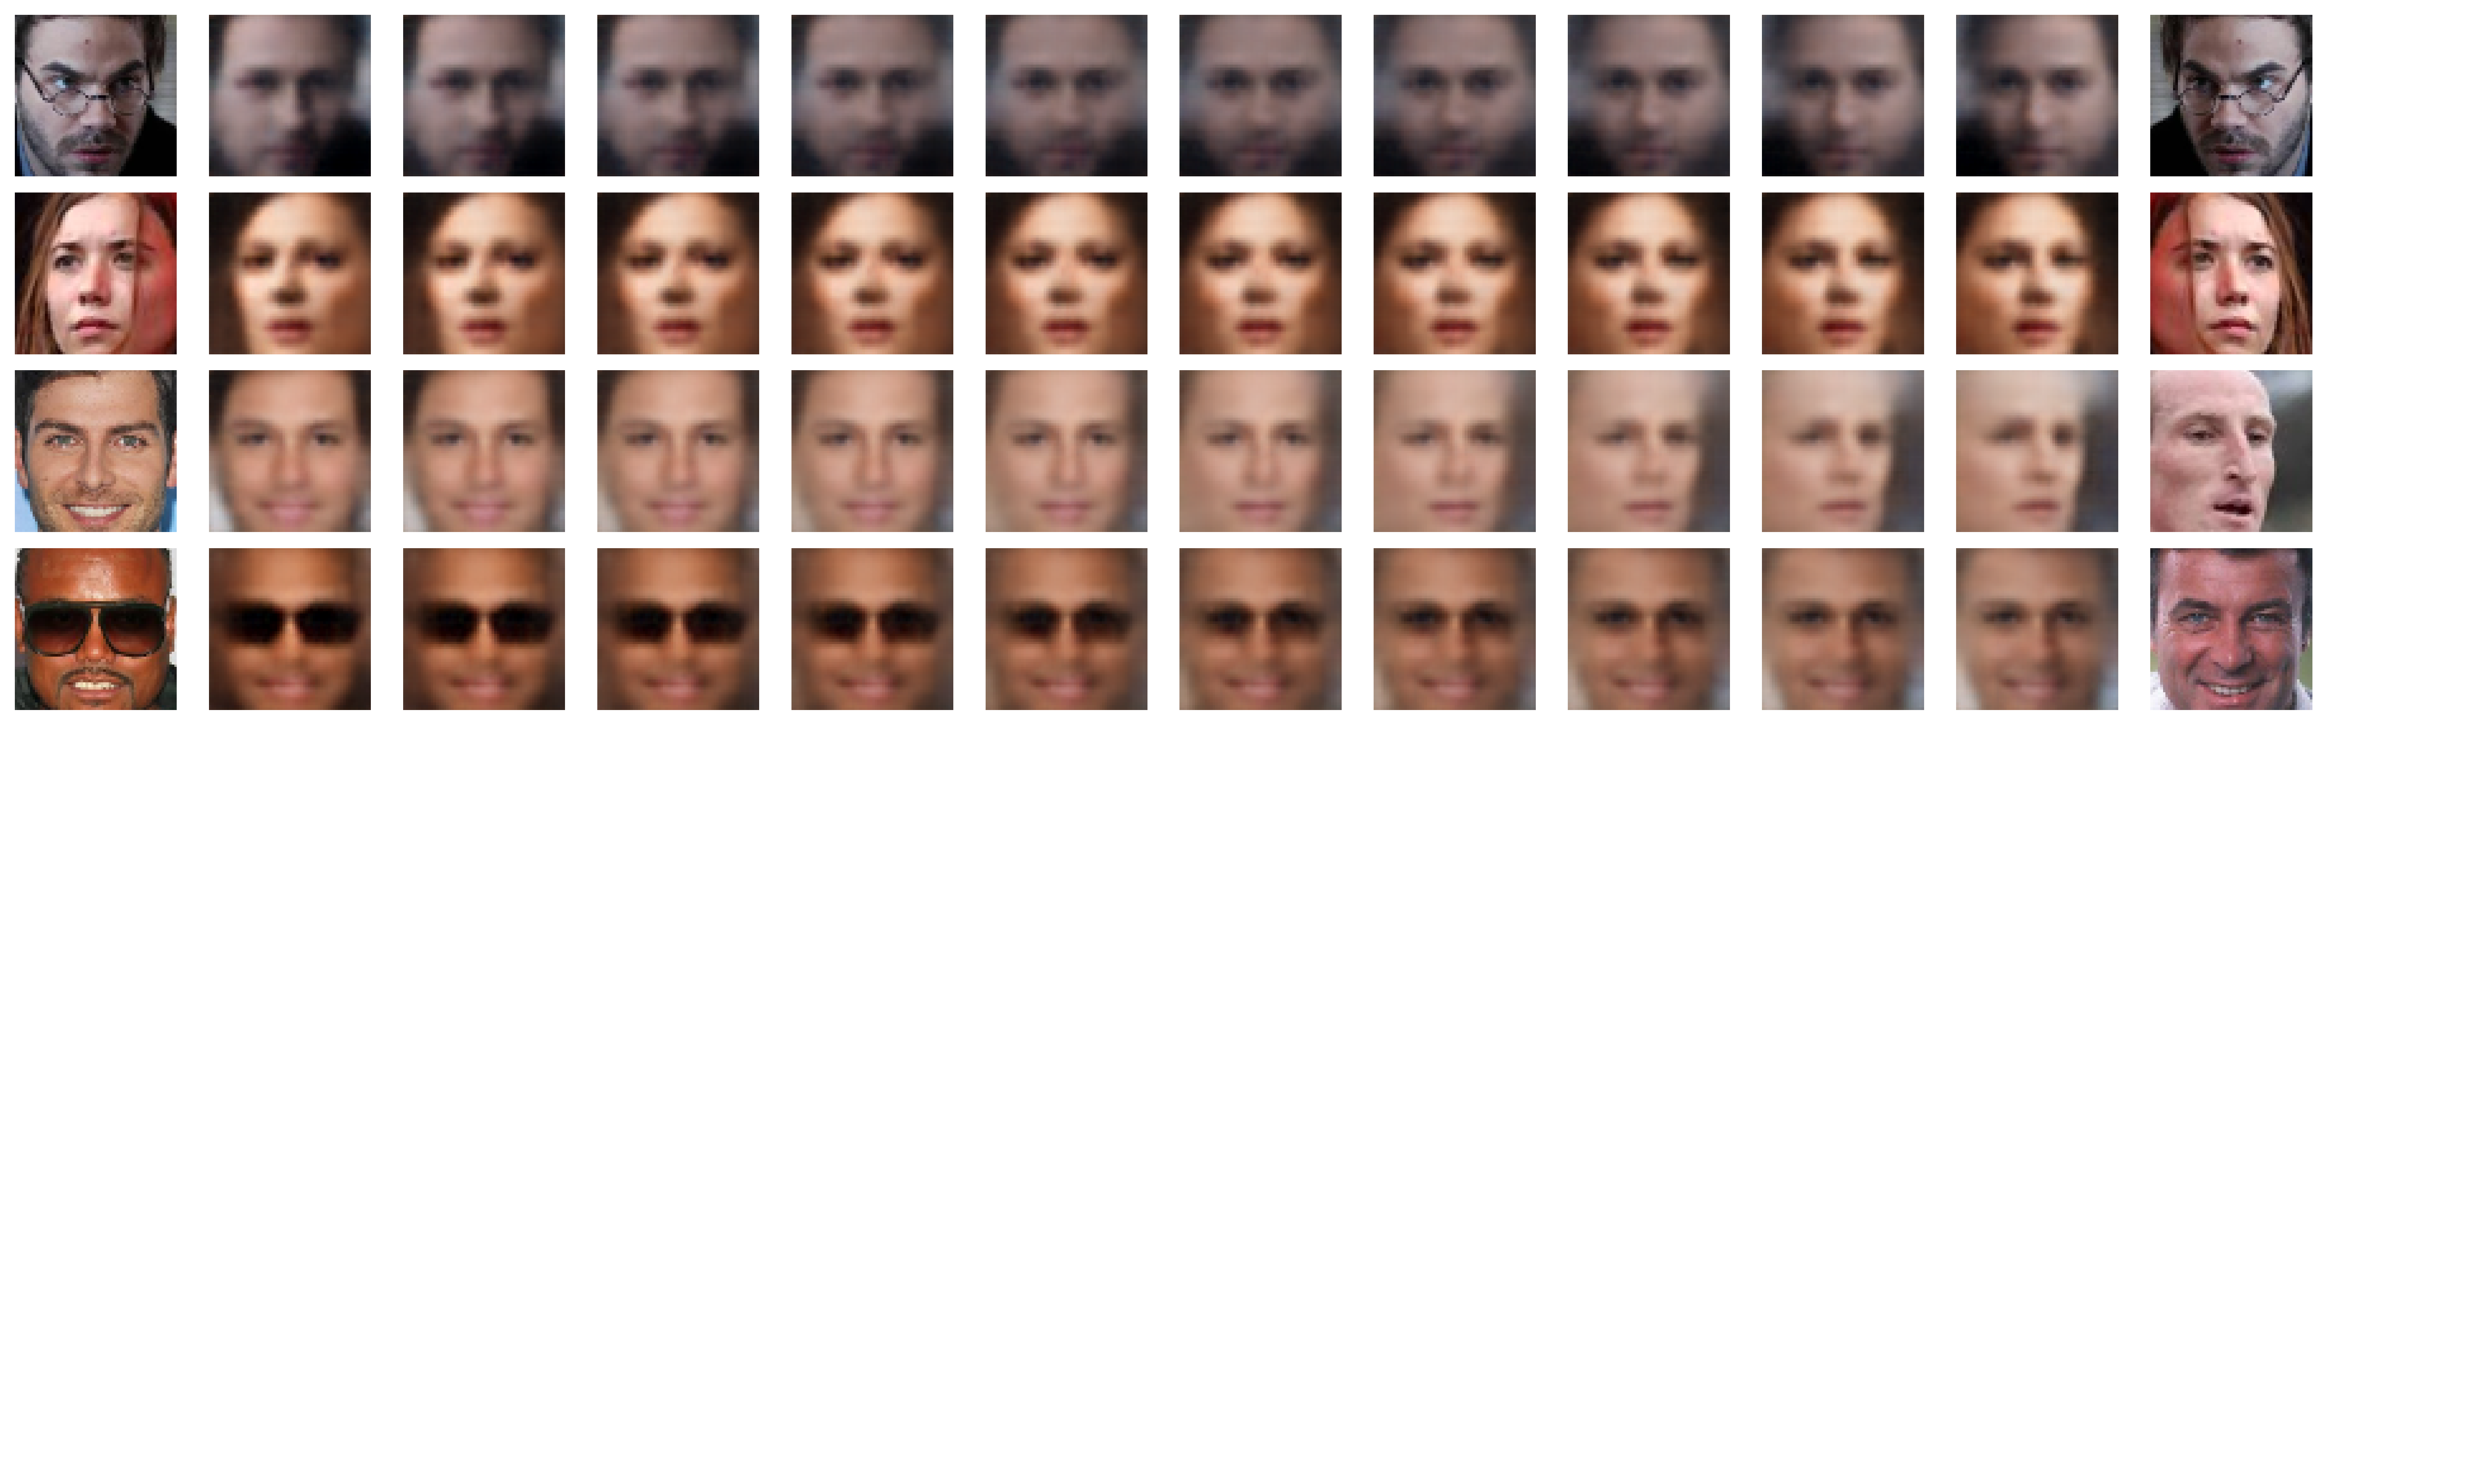
\includegraphics[scale=0.171]{./code/figures/DB-VAE/face_gradient.drawio.pdf}
  \caption{图像渐变效果}
  \label{fig-face-gradient}
\end{figure}

下面代码4-9给出了DB-VAE的代码实现,主要分为模型搭建(编码网络,解码网络),损失函数(隐参数损失,重建损失,二分类交叉熵损失)及网络训练。

\begin{breakablealgorithm}
    \caption{DB-VAE模型}
\begin{pythoncode}
### VAE 参数重采样 ###

def sampling(z_mean, z_logsigma):
    batch, latent_dim = z_mean.shape
    epsilon = tf.random.normal(shape=(batch, latent_dim))
    z = z_mean + tf.math.exp(0.5 * z_logsigma) * epsilon
    return z

### 创建 DB-VAE 模型 ###

class DB_VAE(keras.Model):
    def __init__(self, latent_dim):
        super().__init__()
        self.latent_dim = latent_dim
        # 编码器输出大小,包含隐参数估计mu,logsigma和分类结果y
        num_encoder_dims = 2*self.latent_dim + 1
        self.encoder = make_CNN_classifier(num_encoder_dims)
        self.decoder = make_face_decoder_network()
        
    def encode(self, x):  # 输入图像到编码器中,返回潜空间的参数和二分类的概率
        encoder_ouput = self.encoder(x)
        y_logit = tf.expand_dims(encoder_ouput[:, 0], -1)  # 取输出向量中第0维作为分类概率
        # 潜变量的均值和方差
        z_mean = encoder_ouput[:, 1:self.latent_dim+1]
        z_logsigma =  encoder_ouput[:, self.latent_dim+1:]
        return y_logit, z_mean, z_logsigma
    
    def reparameterize(self, z_mean, z_logsigma):  # VAE重新参数化,从正态分布中取样
        return sampling(z_mean, z_logsigma)
    
    def decode(self, z):
        return self.decoder(z)
    
    def call(self, x):  # 定义该模型的计算过程
        y_logit, z_mean, z_logsigma = self.encode(x)
        z = self.reparameterize(z_mean, z_logsigma)
        recon = self.decode(z)
        return y_logit, z_mean, z_logsigma, recon
    
    def predict(self, x):  # 预测给定的输入x是否是人脸图片
        y_logit, z_mean, z_logsigma = self.encode(x)
        return y_logit
    
dbvae = DB_VAE(latent_dim)
\end{pythoncode}
\end{breakablealgorithm}

\begin{breakablealgorithm}
    \caption{编码部分-卷积网络}
\begin{pythoncode}
n_filters = 12 # 每个卷积层中卷积核的个数

def make_CNN_classifier(n_output=1):
    Conv2D = functools.partial(layers.Conv2D, padding='same', activation='relu')  # padding='same'表示进行零填充
    
    return keras.Sequential([
        Conv2D(filters=1*n_filters, kernel_size=5, strides=2, input_shape=(64, 64, 3)),  # strides为卷积的步长
        layers.BatchNormalization(),
        Conv2D(filters=2*n_filters, kernel_size=5, strides=2),
        layers.BatchNormalization(),
        Conv2D(filters=4*n_filters, kernel_size=3, strides=2),  #  降低卷积核的大小,以提取更多的信息
        layers.BatchNormalization(),
        Conv2D(filters=6*n_filters, kernel_size=3, strides=2),
        layers.BatchNormalization(),
        layers.Flatten(),
        layers.Dense(512, activation='relu'),
        layers.Dense(n_output)
    ])
\end{pythoncode}
\end{breakablealgorithm}
\begin{breakablealgorithm}
    \caption{解码部分-转置卷积网络}
\begin{pythoncode}
n_filters = 12  # 卷积核个数,和编码部分CNN相同
latent_dim = 100  # 隐变量mu维度

def make_face_decoder_network():
    Conv2DTranspose = functools.partial(layers.Conv2DTranspose, padding='same', activation='relu')
    return keras.Sequential([
        # 和上文中的CNN建图过程部分正好相反
        layers.Dense(units=4*4*6*n_filters),  # 上文卷积最后得到图像大小正好是4*4,层数为6N
        layers.Reshape(target_shape=(4, 4, 6*n_filters)),
        Conv2DTranspose(filters=4*n_filters, kernel_size=3, strides=2),
        Conv2DTranspose(filters=2*n_filters, kernel_size=3, strides=2),
        Conv2DTranspose(filters=1*n_filters, kernel_size=5, strides=2),
        Conv2DTranspose(filters=3, kernel_size=5, strides=2)
    ])
\end{pythoncode}
\end{breakablealgorithm}
\begin{breakablealgorithm}
    \caption{VAE损失函数$L_{\text{VAE}} = c\cdot \frac{1}{2}\sum_{j=0}^{k-1}(\sigma_j + \mu_j^2-1-\log\sigma_j) + ||x-\hat{x}||_1$}
\begin{pythoncode}
def vae_loss_func(x, x_recon, mu, logsigma, kl_weight=0.0005):
    """
        x: 输入特征,
        x_recon: 重建输出,
        mu: 编码均值,
        logsigma: 标准差取log的结果,
        kl_weight: 隐参数损失的权系数(正则化系数)
    """
    latent_loss = 0.5 * tf.reduce_sum(tf.exp(logsigma) + tf.square(mu) - 1.0 - logsigma, axis=1)
    reconstruction_loss = tf.reduce_mean(tf.abs(x - x_recon), axis=(1,2,3))
    vae_loss = kl_weight * latent_loss + reconstruction_loss
    return vae_loss
\end{pythoncode}
\end{breakablealgorithm}
\begin{breakablealgorithm}
    \caption{DB-VAE损失函数$L_{total}=  L_y(y, \hat{y}) + \chi_{image}(y)\cdot L_{VAE}$}
\begin{pythoncode}
def debiasing_loss_func(x, x_pred, y, y_logit, mu, logsigma):
    vae_loss = vae_loss_func(x, x_pred, mu, logsigma)
    classification_loss = tf.nn.sigmoid_cross_entropy_with_logits(labels=y, logits=y_logit)
    face_indicator = tf.cast(tf.equal(y, 1), tf.float32)
    total_loss = tf.reduce_mean(
        classification_loss + 
        face_indicator * vae_loss
    )
    return total_loss, classification_loss
\end{pythoncode}
\end{breakablealgorithm}
\begin{breakablealgorithm}
    \caption{DB-VAE训练}
\begin{pythoncode}
### Training the DB-VAE ###

# 超参数配置
batch_size = 32
learning_rate = 5e-4
latent_dim = 100
num_epochs = 15

dbvae = DB_VAE(latent_dim)
optimizer = keras.optimizers.Adam(learning_rate)

# 使用 @tf.function 将Python中的函数,转化为TensorFlow中的计算图,用于计算偏导数
@tf.function
def debiasing_train_step(x, y):
    with tf.GradientTape() as tape:  # 自动求导
        y_logit, z_mean, z_logsigma, x_recon = dbvae(x)
        loss, class_loss = debiasing_loss_func(x, x_recon, y, y_logit, z_mean, z_logsigma)
    grads = tape.gradient(loss, dbvae.trainable_variables)
    optimizer.apply_gradients(zip(grads, dbvae.trainable_variables))
    return loss

all_faces = loader.get_all_train_faces()

for i in range(num_epochs):
    # 重新计算重采样的概率
    p_faces = get_training_sample_probabilities(all_faces, dbvae)
    
    # 获取训练数据集,开始训练
    for j in tqdm(range(loader.get_train_size() // batch_size)):
        (x, y) = loader.get_batch(batch_size, p_pos=p_faces)
        loss = debiasing_train_step(x, y)
\end{pythoncode}
\end{breakablealgorithm}
\section{参考文献}
\begin{enumerate}
    \item 孟德宇。西安交通大学《机器学习》课程PPT, 2023.
    \item Christopher, M. Bishop. Pattern Recognition and Machine Learning, Springer, 2006. 9. Mixture Models and EM.
    \item Auto-Encoding Variational Bayes, Diederik P Kingma and Max Welling, 2013. 9.
    \item Alexander Amini, Ava P. Soleimany, et al. Uncovering and Mitigating Algorithmic Bias through Learned Latent Structure, 2019. 1.
    \item MIT 6.S191 Lib2, 2022.
\end{enumerate}
\end{document}
